\textbf{VIII -- IL SACRIFICIO POSIZIONALE}

\textbf{(o strategico)}

Il sacrificio è, di solito, una potente arma tattica per scardinare la
difesa.

In questo capitolo esamineremo un tipo di sacrificio meno comune, quello
che non si basa sul calcolo delle varianti ma su principi generali di
strategia. I risultati non sono quindi immediati come nel sacrificio
tattico, dove in poche mosse si assiste a un ritorno del materiale o al
matto, ma sono di o¢dine posizionale come la conquista di una colonna,
il dominio di una diagonale ecc.

A ben riflettere abbiamo già fatto conoscenza con sacrifici strategici:
i gambetti!

Il sacrificio di pedone in apertura, infatti, è davvero reale, non ci
sono continuazioni forzate che lo recuperino: il materiale viene
sacrificato per ottenere una maggiore spinta iniziale. Più rari sono i
sacrifici posizionali di pezzi che denotano sempre la mano del giocatore
esperto.

Sono noti alcuni sacrifici di pezzo effettuati nelle prime mosse e
considerati corretti dalla teorie delle aperture, vediamone alcuni:

-- \emph{Gambetto di Re:} \textbf{1.e4 e5 2.f4 exf4 3.¤f3 g5 4.¥c4 g4
5.0-0} (Muzio) \textbf{5... gxf3 6.£xf}3.

-- \emph{Difesa dei due Cavalli:} \textbf{1.e4 e5 2.¤f3 ¤c6 3.¥c4 ¤f6
4.¤g5 d5} (4... ¥c5!? Traxler 5.¤xf7 ¥xf2+) \textbf{5.exd5 ¤xd5 6.¤xf7}
(Fegatello) \textbf{6... ¢xf7 7.£f3+ ¢e6 8.¤c3 ¤b}4.

-- \emph{Difesa Russa:} \textbf{1.e4 e5 2.¤f3 ¤f6 3.¤xe5 d6 4.¤xf7}
(Cochrane) \textbf{4... ¢xf7 5.d4.}

Nella partita che segue, sesta del match per il titolo mondiale,
l'insuperato maestro della combinazione Michael Tal ne effettua uno che
ha fatto versare fiumi d'inchiostro.

Botvinnik--Tal, Mosca 1960 \textbf{(Difesa Est Indiana)}

\textbf{1.c4 ¤f6 2.¤f3 g6 3.g3 ¥g7 4. ¥g2 0-0 5.d4 d6 6.¤c3 ¤bd7 7.0-0
e5 8.e4 c6 9.h3 £d6} costringe il Pd4 a pronunciarsi e minaccia il
guadagno di un pedone con 10... exd4 11.¤xd4 ¤xe4! 12.¤xe4 ¥xd4.

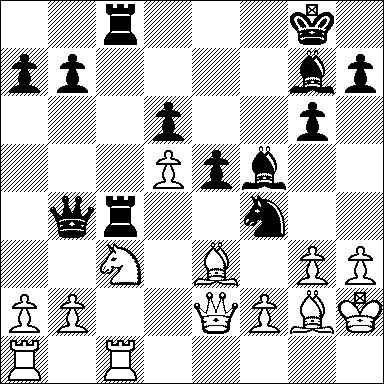
\includegraphics[width=1.40139in,height=1.40139in]{assets/diagrams/image102.png}\textbf{10.d5
¤xd5 11.¤xd5 ¤c5 12.¤e1 ¥d7 13.¤d3 ¤xd3 14. £xd3 ¦fc8 15.¦b1 ch5 16.¥e3
£d4 17.£e2 ¦c4 18.¦fc1 ¦ac8 19.¢h2 f5 20.exf5 ¥xf5 21.¦a1 ¤f4!?}

\emph{diagramma 102}

Una delle mosse più famose di tutta la letteratura scacchistica.

Ecco che cosa scrisse lo stesso Tal di questo sacrificio intuitivo:
\emph{``La controversia e la discussione avviate con questo sacrificio
di Cavallo sono a mio avviso del tutto inutili: questa mossa è buona
perché tutte le altre sono cattive, e se dovesse risultare scorretta,
allora il punto interrogativo non dovrà contrassegnare questo 21° tratto
bensì il 17° tratto del Nero (17... ¦c4). Comunque sia, dopo il
sacrificio suddetto i pezzi neri svilupperanno un grande dinamismo su
tutta la scacchiera (nella fattispecie l'¥g7 finora inattivo), ed il
Bianco dovrà assumersi l'onere di calcolare con la massima esattezza una
miriade di varianti taglientissime''.}

\textbf{22.gxf4 exf4 23.¥d2 £xb2?} un errore che poteva risultare
fatale. La mossa giusta era 23... ¥e5 e ora se 24.¢g1 £xb2 25.¦ab1
\emph{(25.¤d1 ¦xc1)} 25... ¥xb1 26.¦xb1 £c2 27.¦c1 \emph{(27.¥e4 ¦xe4)}
27... £f5 28.£f3 £h5 29.¤e2 ¦c2 con compenso sufficiente grazie al
dominio dell'ala di Donna.

Abbiamo affermato in altra parte che la conoscenza strategica riduce in
modo drastico il calcolo delle varianti, Tal ce lo conferma con queste
illuminanti parole: \emph{``Riflettei circa un quarto d'ora, già una
mossa dopo il sacrificio del pezzo, prima di eseguire questa mossa. Il
motivo è da ricercarsi forse in un errore di calcolo? Oppure il Nero
vuole riesaminare la variante? né l'una né l'altra cosa.}

\emph{Ciò è solo una conferma che il sacrificio in f4 era puramente
intuitivo, e una conferma che non analizzai a tale proposito alcuna
variante ``forzata'', che tendesse cioè al matto o ad altri obiettivi
specifici.''}

\textbf{24.¦ab1 f3 25.¦xb2?} perdendo l'occasione di punire l'errore
commesso dal Nero al 23° tratto. Si doveva giocare 25.¥xf3! ¥xb1 26.¦xb1
£c2 27.¥e4! ¦xe4 28.¤xe4 (28.£xe4 ¥e5+).

\textbf{25... fxe2 26. ¦b3 ¦d4 27.¥e1 ¥e5+ 28.¢g1 ¥f4} vinceva subito
28... ¦xc3! 29.¦bxc3 ¦d1 30.¦c4 ¥b2.

\textbf{29.¤xe2} se 29.¦a1 ¦xc3 30.¦xc3 ¦d1.

\textbf{29... ¦xc1 30.¤xd4 ¦xe1+ 31.¥f1 ¥e4 32.¤e2 ¥e5 33.f4 ¥f6 34.¦xb7
¥xd5 35.¦c7} 35.¦xa7?? ¦xe2 e poi ¥d4+.

\textbf{35... ¥xa2 36.¦xa7 ¥c4 37.¦a8+ ¢f7} è meglio 37... ¢g7 38.¦a7+
¢h6 e il Nero guadagna materiale.

\textbf{38.¦a7+ ¢e6?} in zeitnot (Zeit = tempo, Not = mancanza; termine
tedesco che indica la ristrettezza di tempo) il Nero non si accorge
della difesa escogitata dal Bianco.

\textbf{39.¦a3!} per rispondere a 39... ¥xe2 con 40.¦e3+.

\textbf{39... d5 40.¢f2 ¥h4+ 41.¢g2 ¢d6 42.¤g3 ¥xg3 43.¥xc4 £xc4 44.¢xg3
¢d5 45.¦a7 c3 46.¦c7 ¢d4} il pedone libero decide perciò il Bianco
abbandona.

Un bell'esempio di sacrificio posizionale di Donna si ebbe in una
partita giocata dal Maestro Fide Tullio Marinelli ad Alba Adriatica nel
1992.

Ricordo che nel dopo partita un nugolo di giocatori si accalcò davanti
alla scacchiera ad esaminare la correttezza del sacrificio. Il maestro
romano Marco Lantini mi fece posto dicendomi: ``Vieni a vedere che roba,
incredibile!~''

Marinelli--Hausner, Alba Adriatica 1992 \textbf{(Difesa Est Indiana)}

\textbf{1.d4 d6 2.c4 e5 3.¤f3} la teoria valuta equivalente il gioco
dopo 3.£xe5 £xe5 4.£xd8+ ¢xd8 5.¤c3 c6 6.¤f3 f6 7.g3 ¥e6 8.b3 ¤d7. In
caso di 3.d5, invece, il Nero può operare un'espansione sul lato di Re
con 3... f5.

\textbf{3... exd4} una mossa che non convince del tutto. Il Nero forse
farebbe meglio a mantenere la tensione al centro giocando sia 3... ¤c6
che 3... ¤d7.

\textbf{4.¤xd4 g6} l'intento del Nero di giocare sulla grande diagonale
è palese.

\textbf{5.g3 ¥g7 6.¥g2 ¤e7 7.0-0 0-0 8.¤c3 ¤d7 9.e3} decidendo di
risolvere con un fianchetto di Donna lo sviluppo dell'¥c1. L'idea di
contrapporre l'Alfiere camposcuro all'¥g7 è giustificata. La mancanza di
un Pe7 rende ancora più debole l'arrocco nero in caso di cambio degli
Alfieri su casa nera.

\textbf{9... c6 10.b3 ¤c5 11.¥b2 a5} per completare lo sviluppo il Nero
è stato costretto a indebolire il Pd6. È evidente la necessità di
trovare compensi prima che il Bianco consolidi la posizione e possa
giocare sulla debolezza nera.

\textbf{12.£c2 a4 13.¦ad1 axb3} il Nero ha raggiunto l'obiettivo che si
era proposto. In caso di 14.axb3 può infatti giocare 14... £d6 mentre su
14.¤xb3 la debolezza del Pa2 compensa quella del Pd6.

\textbf{14.¤xb3} di certo meno \emph{naturale} di 14.axb3. Vediamo come
lo stesso Marinelli, sulla rivista \emph{Torre \& Cavallo} giustifica
questo interessante tratto.

``Un tentativo rischioso di conquistare l'iniziativa attraverso le
molteplici possibilità di attacco sul pedone d6, sul ¤c5 e grazie alla
manovra ¤e4. C'è però la minaccia avversaria che incombe sul pedone a2
\ldots{} d'altronde il Bianco aveva progettato questo seguito,
altrimenti non avrebbe giocato ¦ad1 (utile al fine di non ritrovarsi con
l'¥b2 costretto a tornare in c1 in caso di 14... a3) e per finire si
consideri che dopo 14.axb3 £d6 il Nero sarebbe uscito ottimamente
dall'apertura.''

\textbf{14... £c7 15.¤xc5 £xc5 16.£d3} l'idea del Bianco di indebolire
l'arrocco nero mediante il cambio degli Alfieri su casa scura sta per
realizzarsi con la mossa 17.¤e4.

\textbf{16... ¦a6} pensando di impedire 17.¤e4 per 17... ¦b6 e, allo
spostamento della Donna, cade l'Alfiere. Il Nero cade dritto nella
trappola bianca. Sarebbe stato meglio giocare 16... ¥f5.

\textbf{17.¤e4!}

\emph{diagramma 103}

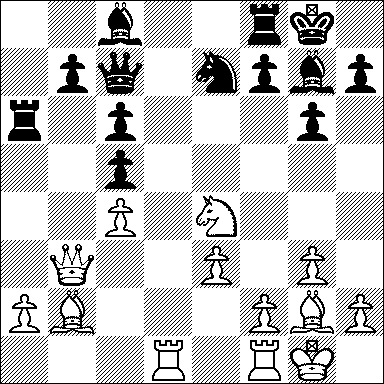
\includegraphics[width=1.40139in,height=1.40139in]{assets/diagrams/image103.png}

\emph{``Audace''} --- commenta Marinelli su \emph{Torre \& Cavallo} ---
\emph{``ma non potevo più tirarmi indietro~\ldots{} già da 16. £d3 avevo
deciso di giocare in questo modo.''}

A questo punto Hausner deve aver capito che le cose non sarebbero andate
come pianificate. Non rimane che verificare la validità del sacrificio.

\textbf{17... ¦b6 18.¥xg7 ¦xb3 19.¥xf8 ¦a3} Marinelli commenta:
\emph{``Il Nero poteva puntare al pedone c4 con 19... ¦b4 ma, in tal
caso, il Bianco avrebbe sfruttato l'impossibilità della ritirata in
ottava giocando ¥h6 e se 20... f5 21.¤g5 (con la minaccia di ra£doppiare
sulla colonna aperta e dare uno scacco mortale in d8) 21... f4 22.¥e4
¥f5 23.¦d3 ¥xe4 24.¤xe4 con attacco vincente''.}

\textbf{20.¥h6} la Torre e un Alfiere non valgono una Donna e da un
punto di vista strettamente materiale il Nero è in vantaggio ma la
debolezza delle case nere e il controllo della colonna \emph{d}
permettono al Bianco di giocare per vincere. Lo sfruttamento del
vantaggio posizionale da parte di Marinelli è esemplare per gioco e
correttezza.

\textbf{20... f5 21.¤f6+ ¢f7 22.¤xh7 ¦xa2 23.¤g5+ ¢e8 24.¥g7 £a5} 24...
¦c2 segue 25.e4.

\textbf{25.¥f3!} con l'idea di mobilitare il pedone ``h''.

\textbf{25... £d4} il guaio del Nero è di non riuscire a far entrare in
gioco la Donna.

\textbf{26.h4 £xc4 27.h5 ¥e6} 27... gxh5 28.¥xh5+ e cala il sipario.
Questa manovra evita che il pedone ``h'' giunga a promozione senza
ostacoli ma non ci sono difese contro la debolezza dell'ottava traversa.

\textbf{28.¦d6 ¥g8 29.h6 ¦c2 30.¦fd1 ¤d5 31.¥xd5 ¤xd5 32.¥f6} il matto
(¦d8\#) è imparabile. Il Nero abbandona.

\textbf{a) Il sacrificio di qualità}

La qualità è la differenza che intercorre tra una Torre e un pezzo
minore.

Questo è anche un ottimo esempio di superiorità dei Cavalli sugli
Alfieri.

Hartston--Mariotti, Olimpiade di Skopje 1972 \textbf{(Partita Viennese)}

\textbf{1.e4 ¤c6} una difesa poco comune che porta il nome di
Nimzowitsch. Mariotti è solito giocare varianti minori e in disuso dove
più che le capacità mnemoniche contano fin dalle prime mosse le capacità
scacchistiche.

\textbf{2.¤c3} il Bianco non accetta la sfida. La continuazione canonica
era 2.d4 ma c'era il rischio di una variante preparata.

\textbf{2... e5} rientrando in una variante minore della partita
Viennese.

\textbf{3.g3} di solito si preferisce spingere in f4, rientrando in
varianti che si confondevano con quelle del Gambetto di Re. Ma, nella
sottile lotta per decidere chi deve indirizzare la partita e in quale
direzione, il Bianco vuol dire la sua.

\textbf{3... ¥c5 4.¥g2 h5} una novità teorica tipica dello stile del
Grande Maestro italiano. Con questa spinta a¢dita il Nero infrange le
aspirazioni del Bianco a giocare in modo posizionale e punta ad aprire
la colonna ``h''. In altra parte abbiamo visto che la spinta di rottura
del pedone ``h'', in caso di fianchetto è buona strategia ma i canoni
vogliono che si debba intraprendere un attacco solo dopo aver completato
lo sviluppo. Questa spinta va contro le regole comunemente accettate e
perciò l'intuizione di Sergio Mariotti è maggiormente rimarchevole.

\textbf{5.¤f3} sviluppa un pezzo e controlla in h4 ma Mariotti va dritto
per la sua strada.

\textbf{5... h4 6.¤xh4}

\emph{diagramma 104}

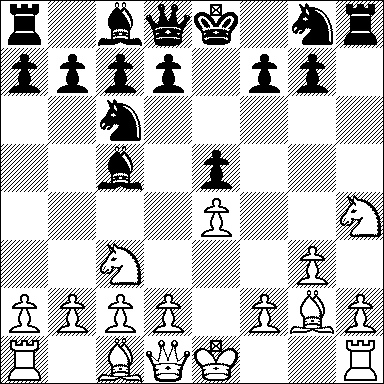
\includegraphics[width=1.40139in,height=1.40139in]{assets/diagrams/image104.png}

\textbf{6... ¦xh4} pare incredibile che il Nero possa sacrificare la
qualità dopo appena sei mosse di gioco!

\textbf{7.gxh4 £xh4} l'iniziativa nera compensa ad usura la qualità
sacrificata. Questa partita è un ottimo esempio di tecnica scacchistica
e perciò merita di essere studiata con particolare attenzione.

\textbf{8.d4} non essendo il caso di arroccare corto né di giocare 8.£e2
(o 8.£f3) per 8... ¤d4, questa mossa è praticamente forzata.

\textbf{8... ¥xd4} a 8... ¤xd4 il Bianco poteva replicare con la
semplice 9.¤a4 seguita da 10.¥e3 e l'iniziativa del Nero svanisce come
nebbia al vento.

\textbf{9.£e2 ¥xc3+!} una mossa che denota la mano del maestro e per
almeno due ragioni: la prima è che pochi si sarebbero privati di questo
splendido Alfiere e la seconda è la capacità di cambiare piano di gioco.
Le prime mosse del Nero potevano far credere a una partita di attacco e
invece il Nero cambia le carte in tavola, chiude la posizione, e si
appresta a far valere la superiorità posizionale che i numerosi buchi
dello schieramento bianco gli conferiscono; buchi che valorizzano i due
Cavalli in possesso del Nero.

\textbf{10.bxc3 d6 11.0-0 g5} naturalmente non si può permettere f4.
L'apertura delle linee favorisce sempre chi ha la coppia degli Alfieri.

\textbf{12.£e3 f6 13.£g3 £h7 14.¥f3 ¤ge7 15.¦e1} protegge il Pe4 e
prepara il cambio degli Alfieri campo chiaro; desiderio del tutto
legittimo perché quello del Bianco, a causa del Pe4, è cattivo, mentre
quello del Nero è buono.

\textbf{15... ¤g6 16.¥e3 ¢e7} si prepara a portare in gioco anche la
Torre, destinata alla colonna h.

\textbf{17.c4} tentando di reagire ad ovest ma Mariotti non molla la
presa.

\textbf{17... b6 18.c5 bxc5 19. c3 ¤f4 20.¥g4 ¥xg4 21.£xg4 ¦h8 22.h4 £g8
23. ¥xf4} pe¢de di schianto 23.hxg5 £h7 24.gxf6+ ¢d8 e non c'è modo di
evitare il matto, però questa mossa costa un pedone.

\textbf{23... ¦xh4 24.£g2 exf4 25.e5 ¤xe5 26.£d7 ¦g4+ 27.¢f1 £c4+ 28.¦e2
¢d7 29.£e4 f3 30.£xc4 ¤xc4 31.¦c2 ¦g2 32.¦e1 f5 33.¦2e2 ¢c6 34.} il
Bianco abbandona.

In questa partita, decima della finale del campionato del mondo,
l'indiscusso maestro della partita posizionale Tigran Petrosian,
campione del mondo dal 1963 al 1969, sacrifica entrambe le qualità per
l'iniziativa. Petrosian tendeva a tenere la partita sempre sotto
controllo cercando di non lasciare nulla al caso (per questo fu
irriverentemente definito ``il coniglio più forte del mondo'') e i
sacrifici cui a volte ricorre, come nel caso che segue, sono sempre
squisitamente posizionali. Il colpo tattico finale, inevitabile
conclusione di una partita vinta strategicamente, è molto bello anche se
non ha nulla di aleatorio.

Petrosian--Spassky, Mosca 1966 \textbf{(Est Indiana)}

\textbf{1.¤f3 ¤f6 2.g3 g6 3.c4 ¥g7 4.¥g2 0-0 5.0-0 ¤c6 6.¤c3 d6 7.d4 a6}
evita le complicazioni che derivano da 7... e5 8.d5 ¤e7 9.c5!,
favorevoli al Bianco.

\textbf{8.d5 ¤a5 9.¤d2 c5 10.£c2 e5 11.b3} l'alternativa 11.£xe6 ¥xe6
conduce all'uguaglianza perché i bianchi non possono impedire d5.

\textbf{11... ¤g4 12.e4} era più forte 12.¥b2 f5 13.¦ae1 seguita da ¤d1
e f4.

\textbf{12... f5 13.exf5 gxf5 14.¤d1 b5} per rendere possibile
l'eventuale passaggio sull'ala di Re della Torre via a7.

\textbf{15.f3 e4 16.¥b2} non va 16.¦b1 per 16... ¥d4+ 17.¢h1 ¤xh2! ed è
difficile parare l'attacco nero.

\textbf{16... exf3 17.¥xf3 ¥xb2 18.£xb2 ¤e5 19.¥e2 f4} necessaria per
evitare che il Bianco controlli la casa f4 con la manovra ¤e3-g2, con un
chiaro vantaggio posizionale.

\textbf{20.gxf4 ¥h3} il Nero si lascia sfuggire la mossa migliore: 20...
¦xf4!

\textbf{21.¤e3!}

\emph{diagramma 105}

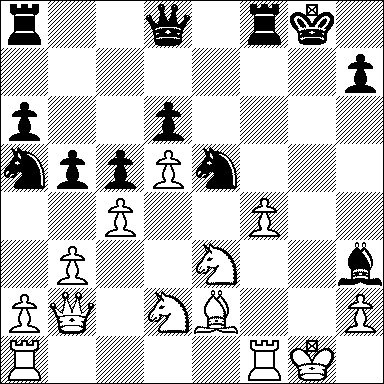
\includegraphics[width=1.40139in,height=1.40139in]{assets/diagrams/image105.png}

Il Bianco sacrifica la qualità per ottenere il controllo delle case
bianche. Ora la presa di Torre lascia il Bianco in vantaggio, vediamo:
21... ¦xf4 22.¦xf4 £g5+ 23.¦g4 (23.¢h1 £xf4 24.¦g1+) 24... ¤xg4 25.¥xg4
£xg4+ 26.¢h1 con la terribile minaccia ¦g1.

\textbf{21... ¥xf1} forse Spassky avrebbe fatto bene a seguire i
consigli di Botvinnik che una volta disse: \emph{``Se Petrosian
sacrifica un pezzo non lo prendere, se lo sacrifico io prima verifica le
varianti e poi prendilo, se lo sacrifica Tal prima prendilo e poi
verifica le varianti''.}

\textbf{22.¦xf1 ¤g6 23.¥g4 ¤xf4} maggiore resistenza offriva 23... £f6
24.¥e6+ ¢g7 25.£xf6+ ¦xf6 26.f5 e la minaccia ¤e4 è molto forte.

\textbf{24.¦xf4 ¦xf4 25.¥e6+ ¦f7} se 25... ¢f8 26.£h8+ ¢e7 27.£xh7+ con
attacco imparabile.

\textbf{26.¤e4} il Nero si difende dopo 26.¤f5 £g5+ 27.¢h1 £xf5!

\textbf{26... £h4 27.¤xd6 £g5+} dopo 27... £e1+ 28.¢g2 non ci sono più
scacchi.

\textbf{28.¢h1 ¦aa7 29.¥xf7+ ¦xf7}

\emph{diagramma 106}

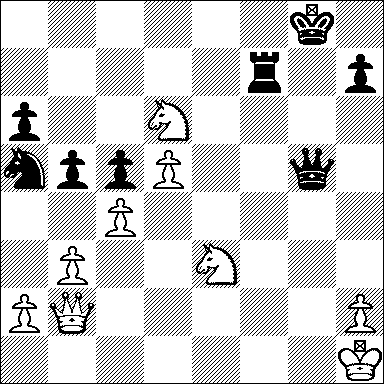
\includegraphics[width=1.40139in,height=1.40139in]{assets/diagrams/image106.png}

\textbf{30.£h8+!!} una degna conclusione. Dopo 30... ¢xh8 31.¤xf7+ e
32.¤xg5 il Bianco rimane con un pezzo in più, pertanto il Nero
abbandona.
